\documentclass[11pt, a4paper]{article}

\usepackage{amsmath}
\usepackage{amsfonts} %Matheschriften
\usepackage{amssymb} %Mathesymbole
%\usepackage{mathptmx} % Einstellung für Schriften und Sonderzeichen in mathematischen Umgebungen
                        % ändert SChriftfont
\usepackage{wasysym} % Stellt diverse Sonderzeichen bereit
\usepackage{siunitx}
\usepackage{float}
\usepackage{microtype}
\usepackage{graphicx}
\usepackage{hyperref}
\usepackage{xcolor}
\usepackage[section]{placeins}
% allows for temporary adjustment of side margins
\usepackage{changepage}
\usepackage{rotating}
\usepackage{physics}

\usepackage[ngerman]{babel}
\addto\captionsngerman{%
 \renewcommand{\abstractname}{Einleitung}}

 \DeclareSIUnit\year{a}
\DeclareSIUnit\electron{e}
 \DeclareSIUnit\atomicmassunit{amu}

\title{Versuch 3: Radioaktivität}
\author{Team 4-11: Jascha Fricker, Benedict Brouwer}

\begin{document}
    \maketitle

    \tableofcontents

    \newpage

    \section{Theorie}
    \subsection{Zerfallsgleichungen}
    Die Zerfallsgleichungen beschreiben die Anzahl der Kerne N sowie die Aktivität $A$ verbunden mit der Halbwertszeit $T$
    \begin{align}
        N(t) &= N_0 \cdot e^{- \lambda t} \label{eq:zerfälleNachZeit} \\
        T &= \frac{\ln 2}{\lambda} \label{eq:Halbwertszeit}  \\ 
        A(t) &= - \dv{N(t)}{t} = \lambda N(t) \label{eq:Aktivität-halb}
    \end{align}
    
    \subsection{Zerfallreihen}
    In der Abbildung \ref{fig:zerf} können die Zerfallsenergien und Zerfallsreihen einiger der in diesem Praktikum genutztden radioaktiven Stoffe gefunden werden.

    \begin{figure}[!h]
        \centering
        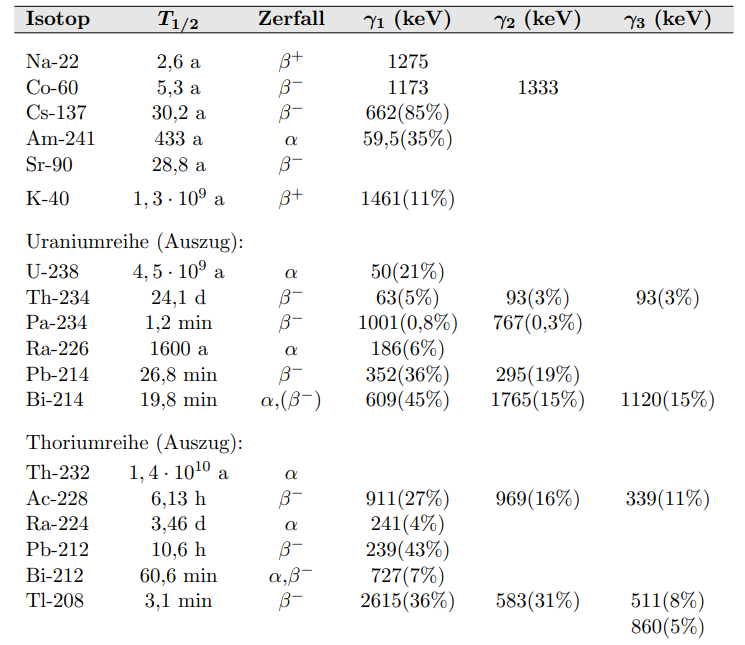
\includegraphics[width=\textwidth]{Screenshot 2023-03-14 5.37.47 PM.png}

        \caption{$\gamma$-Energieen einiger Stoffe, Quelle: \cite{RAD}}
        \label{fig:zerf}
    \end{figure}
    
    \section{Versuchsaufbau und Druchführung}

    In diesem Experiment werden mehrere Radioaktive Proben vermessen. Dafür wird die Probe vor ein NaI Kristall gestellt. Die Emittierten Photonen werden durch einen Photomultiplier verstärkt. Ein Computerprogramm zählt die Ereignisse und ordnet sie nach der Energie in verschiedene Kanäle ein. Der Aufbau ins in Abbildung \ref{fig:aufbau} dargestellt. So ensteht ein Radioaktives Spektrum. Zuerst wurde die Energiemessung durch 3 Kallibrationsporben kallibriert. Anschließend wurden verschiedene Proben gemessen.
    
    \begin{figure}
        \centering
        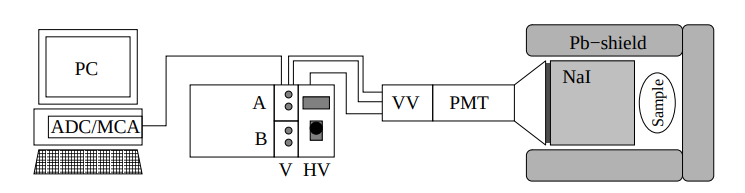
\includegraphics[width=0.8\textwidth]{Screenshot 2023-03-14 5.37.15 PM.png}
        \caption{Versuchsaufbau}
        \label{fig:aufbau}
    \end{figure}

    \section{Ergebnisse}
    \subsection{Kallibrierung}
    Um die Energie der einfallenden Teilchen zu berechnen ist es zuerst nötig, den NaI-zähler zu kallirieren. Dazu wurden die Spektren von Cs-137, Na-22 und Co-60 gemessen und dessen Peaks bestimmt \ref{fig:Kalibspektren}. 
    Anschliesend wurden die Kanalnummern $n$ der Peaks mit den charakteristischen Energien als auch der charakteristischen Energien von Doppelereignissen der einzelnen Proben in Graph \ref{fig:Kanal-Energie} geplottet und mittels einer Ausgleichsgeraden die Kallibrierungskurve bestimmt:
    \begin{align}
        E(n) = 3,052(73) \cdot n - 27.1(31) KeV
    \end{align}
    



    \begin{figure}[!h]
        \centering
        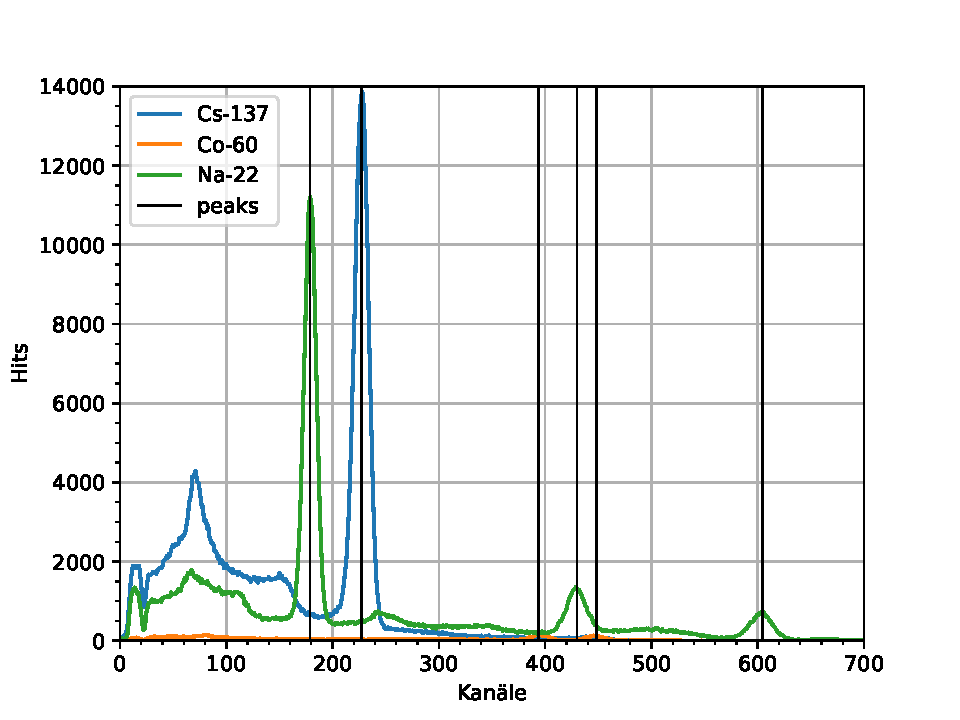
\includegraphics[width=\textwidth]{Plots/Kalibspektren.pdf}

        \caption{Spektren von Cs-137, Na-22 und Co-60 zur Kallibrierung}
        \label{fig:Kalibspektren}
    \end{figure}

    \begin{figure}[!h]
        \centering
        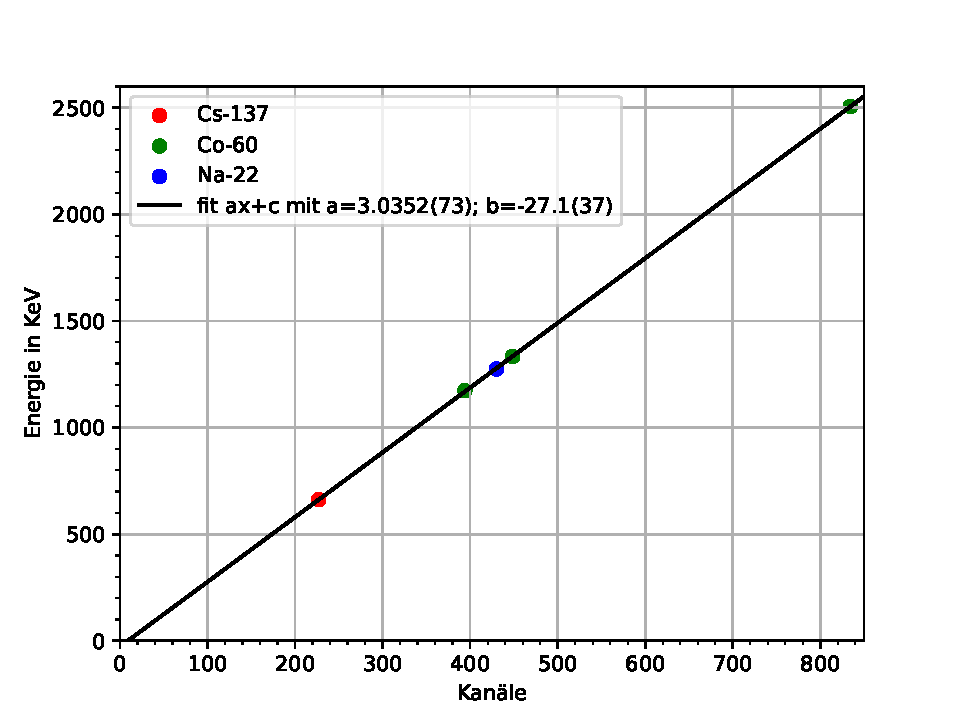
\includegraphics[width=\textwidth]{Plots/Kanal-Energie.pdf}

        \caption{Kalibrierungskurve des NaI-Zählers}
        \label{fig:Kanal-Energie}
    \end{figure}

    \subsection{Strahlenbelastung durch die Cs-137 Probe in einem Jahr}
    Die untersuchte Cs-137 Probe besaß 1992 eine Aktivität $A = 133 \si{\kilo\becquerel}$. Seit 1992 ist etwa die Halbwertszeit von 30,2 Jahren vergangen. Also ist die Aktivität zur Zeit des Experiments $A(2023) = 166.5 \si{\kilo\becquerel}$.
    Um die Strahlenbelastung auf einen Mensch (Rechteck der Form $0,3\si{\meter} \cdot 1,7 \si{\meter}$) zu berechnen, wird zunächst der Raumwinkel abgeschätzt mit $\Omega_{M} = \frac{A_{M}}{4\pi r^2} = 0,041$.
    Daraus folgt für die absorbierte Strahlenenergie bei Annahme vollständiger Absorption und vernachlässing der Aktivitätsänderung im Laufe des Jahres:
    \begin{align}
        E_{M_a} \approx 167 \si{\kilo\becquerel}\cdot 1 \si{\year} \cdot 0,85 \cdot 662 \si{\kilo\electron\volt} \cdot e \cdot \Omega_{M} \approx 0,0189 \si{\joule}
    \end{align}
    Für einen 65 \si{\kilo\gram} schweren Menschen entspricht dies einer Strahlenbelastung von $\frac{E_{M_a}}{65\si{\kilo\gram}} = 0.291\si{\milli\sievert}$
    \subsection{Kaliumcarbonat}
    In diesem Versuchsteil wurde das Spektrum einer Kaliumcarbonatprobe ($K_2CO_3$) wie in Graph \ref{fig:Kaspektrum} zu sehen bestimmt. Wie zu erwarten ist ein Peak bei $1445(26) \si{\kilo\electron\volt}$ zu sehen ist was mit Fehlerintervall mit dem Theoriewert von $1461 \si{\kilo\electron\volt}$ \ref{fig:zerf} übereinstimmt.
    Im Peak sind bei einem Messzeitraum von 10 Minuten $2114(46)$ Ereignisse registriert worden. Mit diesem Wert lässt sich mit 
    \begin{align}
        N_{K} = \frac{m}{2 \cdot M_{K} + M_{C} + 3 \cdot M_{O}} = 4.363 \cdot 10^{23}
        N_{K-40} = \frac{0,0001 \cdot m}{2 \cdot M_{K} + M_{C} + 3 \cdot M_{O}} = 4.363 \cdot 10^{19}
    \end{align}
    Wobei $M_{K} = 39 \si{\atomicmassunit}, M_{C} = 12 \si{\atomicmassunit}, M_{O} = 16 \si{\atomicmassunit}$ die Masse $m = 0,1 \si{\kilo\gram}$ und die Tatsache, dass nur 0,01\% der Nuklide K-40 Nuklide sind, verwendet wurde.

    K-40 hat eine Halbwertszeit von $T_{0,5}=1,28 \cdot 10^{9} \si{\year}$ \ref{fig:zerf}. Daraus folgt mit den Formeln \ref{eq:Halbwertszeit} und \ref{eq:zerfälleNachZeit}
    \begin{align}
        \lambda = 1,760 \cdot 10^{-17} \si{1\per\second}
        A_{theo} = 767.9  \si{\becquerel}
    \end{align}
    Aus den gemessenen Daten folgt mit \ref{eq:Aktivität-halb} für die Aktivität $A=3.52 \si{\becquerel}$. Dieser große Untersched, lässt sich vermutlich erklären durch die Tatsache, dass nur ein kleiner Teil der Strahlung vom NaI-Zähler detektiert wird.
    \begin{figure}[!h]
        \centering
        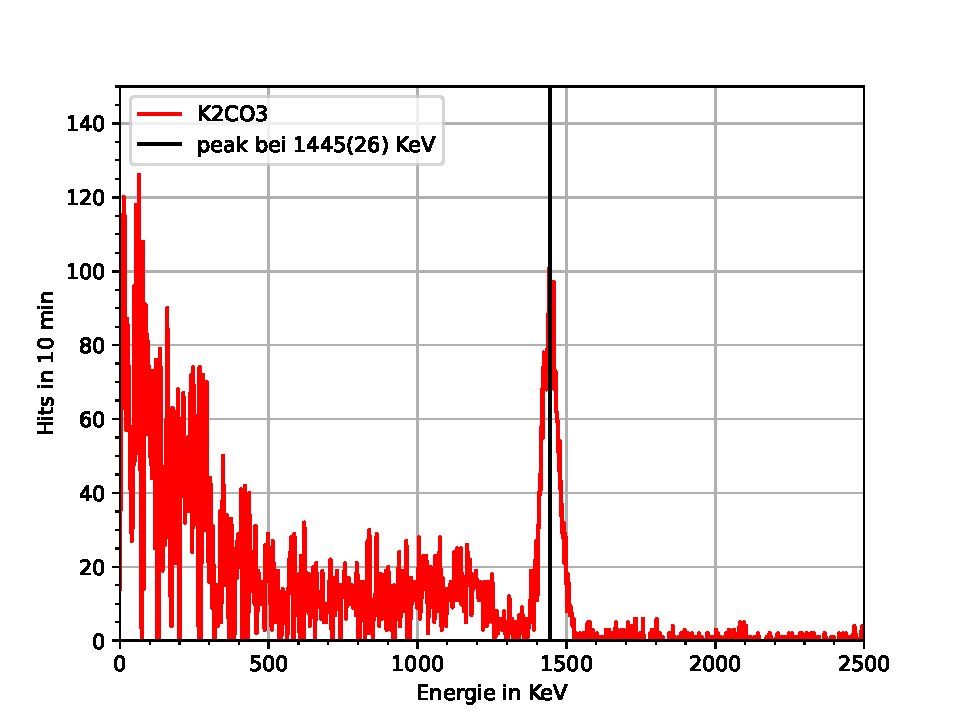
\includegraphics[width=\textwidth]{Plots/K2CO3.pdf}

        \caption{Kaliumcarbonatspektrum abzgl. Hintergrundstrahlung}
        \label{fig:Kaspektrum}
    \end{figure}


    \subsection{Hintergundstrahlung}
    Um die Hintergundstrahlung zu bestimmen wurden je 10 min mit und ohne Bleiabschirmung und ohne Probe gemessen. Die zwei Spektren wurden in Abbildung \ref{fig:hintergrund} geplottet.
    \begin{figure}[!h]
        \centering
        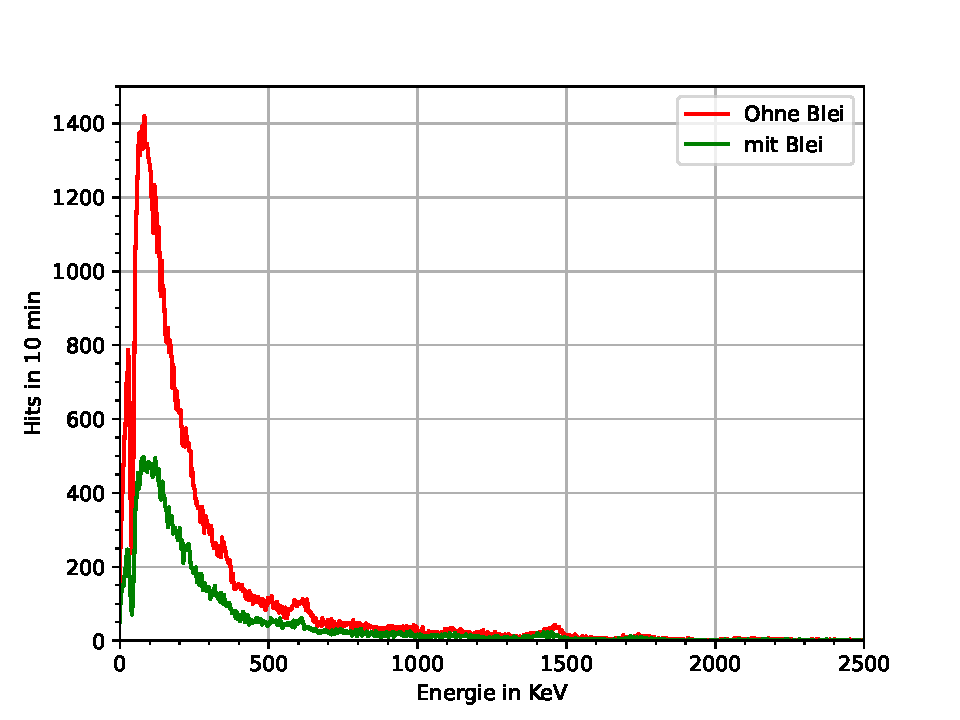
\includegraphics[width=\textwidth]{Plots/Untergrund.pdf}
        \caption{Hintergundstrahlung}
        \label{fig:hintergrund}
    \end{figure}
    Es kann gut erkannt werden, dass das Blei einen großen Teil der Hintergrundstrahlung abschirmt.

    \subsubsection{Strahlenbelastung Hintergrundstrahlung}
    Durch die Abmessungen des Kristalls $d = h = 7,52 \si{\centi\metre}$ und dessen Dichte $p = 3,7 \si{\gram\per\cubic\centi\metre}$ kann die Masse $m$ des Kristalls berechnet werden.
    \begin{align}
        m = p \cdot \pi \cdot \frac{d^2}{4} \cdot h =  1,24 \si{\kilogram}
    \end{align}
    Die gemessene Summe aller Hits ohne Bleiabschirmung in den $t = 10$ min $N_{Hintergrund} = 101110$. Durch die Faustformel ergibt dies etwa $ E = 10 \si{\giga\electronvolt}$. Aus genauer Berechnung ergeben sich $E = 31,1 \si{\giga\electronvolt}$. Wir rechnen aber mit erster Angabe weiter. Es gilt
    \begin{align}
        \frac{D}{t} = \frac{E}{mt} = 67,9 \si{\micro\sievert\per\year} \label{eq:HintergrundZuSiv}
    \end{align}


    \subsection{Strahlenbelastung Gras}
    Abbildung \ref{fig:gras} zeigt die Strahlung einer Probe aus getrocknetem Gras, die in Bayern nach der Tchernobyl-Katastrophe gesammelt wurde. Hier sind klar die Peaks von $^{40}K$ und $^{137}Cs$ zu erkennen.
    \begin{figure}[!h]
        \centering
        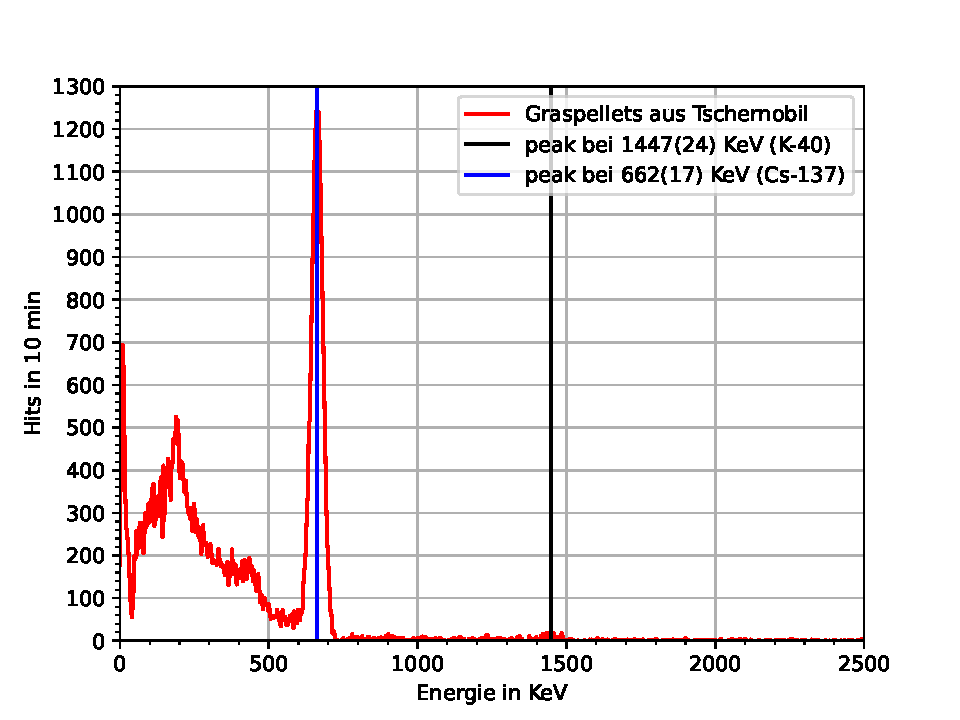
\includegraphics[width=\textwidth]{Plots/Tschern.pdf}
        \caption{Strahlung Grasprobe Hintergundsstrahlungkorrigiert}
        \label{fig:gras}
    \end{figure}
    Wenn die gesammte Hits mit Energien programmatisch summiert werden, kommt man auf eine vom Detektor absorbierte Energie von $E = 23,8 \si{\giga\electron\volt}$ in 10 Minuten. Wir nehmen an, dass der Detektor etwa ein 6-tel der gesammten emittierten Strahlung absorbiert hat und ein Mensch etwa $m = 80 \si{\kilogram}$ wiegt. Außerdem wird die Abnahme der Aktivität innerhalt einer Woche vernachlässigt. Für die Energiedosis folgt
    \begin{align}
        D = \frac{6 E}{m} \frac{\text{Woche}}{10 \si{\min}} = 48 \si{\nano\sievert}
    \end{align}
    in einer Woche.



    \subsection{Uran und Thorium}
    Das Spektrum von Uran wurde in Abbildung \ref{fig:uran} und das von Thorium in \ref{fig:thor} geplottet. In diesen können verschiede Linien erkannt werden, die in Tabelle \ref{tab:uran} mit den wahrscheinlich zugehörigen Elementen aufgeführt werden. Die Enerigewerte wurden mit denen in Abbildung \ref{fig:zerf} gematcht.

    \begin{table}
        \centering
        \begin{tabular}{c|c||c|c}
            \multicolumn{2}{c}{Uran} & \multicolumn{2}{c}{Thorium} \\ \hline
            Energie in $\si{\kilo\electron\volt}$ & Isotop & Energie in $\si{\kilo\electron\volt}$ & Isotop \\ \hline
            77 & Blei & 74 & Blei \\ \hline
            177 & Ra-226 & 232 & Pb-212 \\ \hline
            757 & Pa-234 & 332 & Ac-228 \\ \hline
            996 & Pa-234 & 586 & Ti-208 \\ \hline
            & & 929 & Ac-228 \\ \hline
            & & 1582 & Ac-228 + Ti208\\ \hline
            & & 2557 & Ti- 208

            
        \end{tabular}
        \caption{Isotope der Uran- und Thoriumproben}
        \label{tab:uran}
    \end{table}

    \begin{figure}[!h]
        \centering
        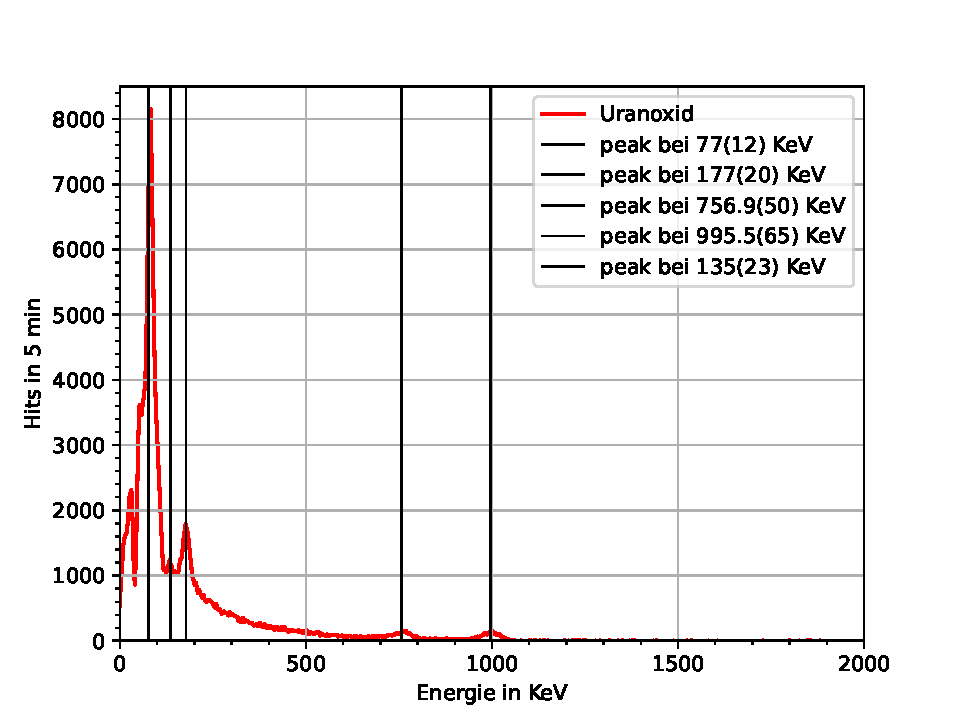
\includegraphics[width=\textwidth]{Plots/Uranox.pdf}
        \caption{Uran}
        \label{fig:uran}
    \end{figure}

    \begin{figure}[!h]
        \centering
        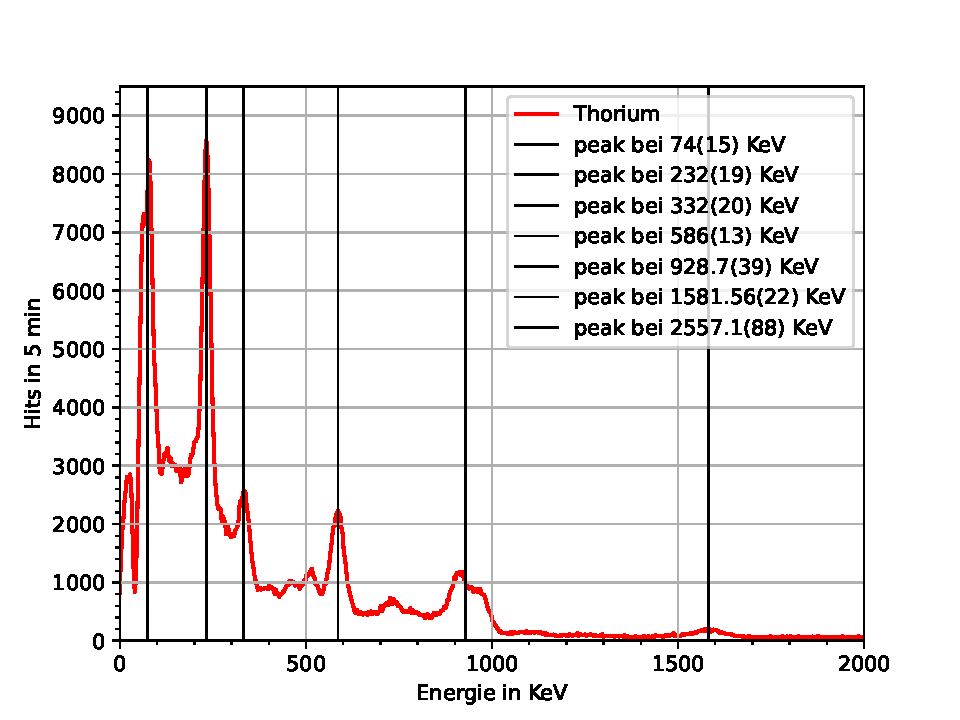
\includegraphics[width=\textwidth]{Plots/Thorium.pdf}
        \caption{Thorium}
        \label{fig:thor}
    \end{figure}

    

    
    \subsection{Wecker}
    In diesem Versuchteil wurde zunächst das Spektrum eines Weckers mit leuchtenden Zeigern aufgenommen um zu bestimmen welche Isotope diese zum leuchten bringen.
    Dazu wurden den Peaks aus Graph \ref{fig:Wecker} die passenden Isotope zugeordent, wie in Tabelle \ref{tab:Weck} zunsehen ist.

    \begin{table}
        \centering
        \begin{tabular}{c|c|c}
            
            Energie des Peaks in $\si{\kilo\electron\volt}$ & charakteristische Energie in $\si{\kilo\electron\volt}$ & Isotop \\ \hline
            65(19) & 77 & Blei \\ \hline
            181(20) & 186 & Ra-226 \\ \hline
            237(19) & 241 & Ra-224 \\ \hline
            292(18) & 295 & Pb-214 \\ \hline
            351(16) & 352 & Pb-214 \\ \hline
            614(12) & 609 & Bi-214 \\ \hline
            779(56) & 767 & Pa-234 \\ \hline
            1118(56) & 1120 & Bi-214 \\ \hline
            1388(47) & 1377 & Bi-214 + Pa-234 \\ \hline
            1744(23) & 1765 & Bi-214 \\ \hline
            2164(66) & 2116 & Bi-214 + Pb-214 \\ \hline


            
        \end{tabular}
        \caption{Isotope des Weckers}
        \label{tab:Weck}
    \end{table}


    \begin{figure}[!h]
        \centering
        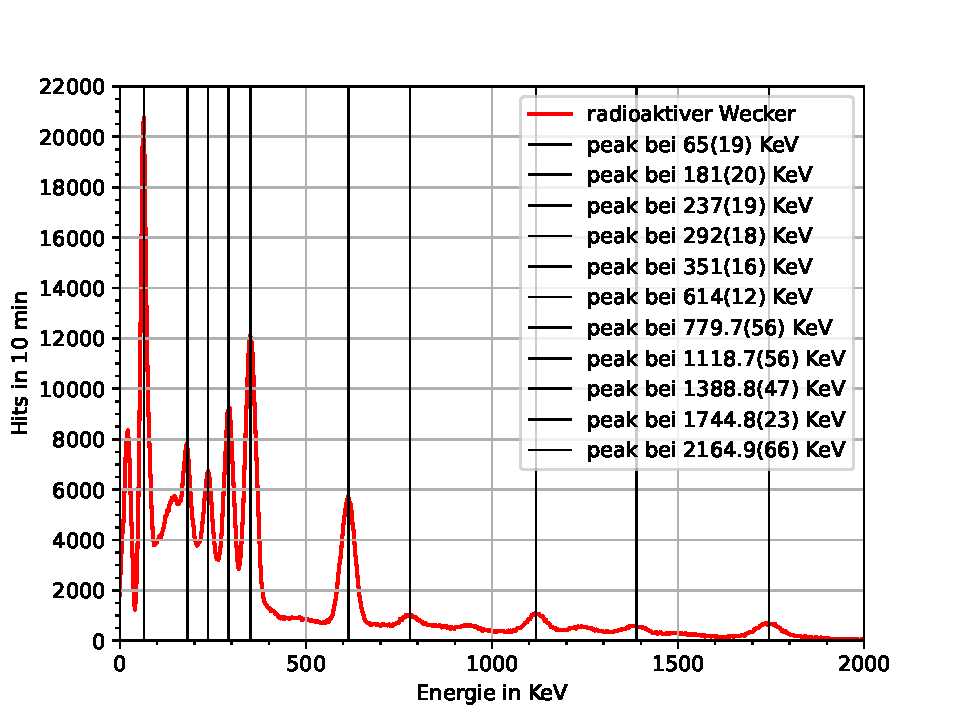
\includegraphics[width=\textwidth]{Plots/Wecker.pdf}
        \caption{Radioaktiver Wecker}
        \label{fig:Wecker}
    \end{figure}

    \subsection{Höhenstrahlung}
    Um Höhenstrahlung welche aus sehr viel höher energeitschen Teilchen besteht zu detektieren muss zunächst der NaI-Zähler erneut kallibriert werden. 
    Dazu wird das Co-60 Spektrum in einem anderen Spannungsbereich aufgenommen (siehe \ref{fig:Co-60spekt}). Mit den Kanalnummern $n$ der Peaks und den bekannten charakteristischen Energien des Co-60 kann nun erneut eine Kallibrierungskurve \ref{fig:Höhenkalib} erstellt werden:
    \begin{align}
        E(n) = 48,80(46) \cdot n + 8(17)
    \end{align}
    Nun wurde das Spektrum der Höhenstrahlung für 2 Stunden gemessen und in Graph \ref{fig:Höhenspekt} geplottet. Die Ereignisse der einzelnen Kanäle in hunderter Schritten sind in Tabelle \ref{tab:Höhenereig} veranschaulicht.
    Dabei wurde Kanal 0-99 vernachlässigt, da dort hauptsächlich die Strahlung radioaktiver Nukleide auftritt. Insgesamt wurde im Messzeitraum eine aufsummierte Energie von $2,219(26) \cdot 10^{11} \si{\electron\volt}$ detektiert.
    Unter der Annahme, dass ein Kilogramm Detektor gleich viel Absorbiert wie ein Kilogramm Mensch kann daraus mit Formel \ref{eq:HintergrundZuSiv} die Strahlenbelastund der Höhenstrahlung berechnet werden zu $E = 0,1225(14) \si{\milli\sievert\per\year}$
    Dieser Wert ist verglichen mit dem Literaturwert ($E = 0,3 \si{\milli\sievert\per\year}$) zwar etwas hoch, liegt aber in der gleichen Größenordnung \cite{cosmic_radiation}.


    \begin{figure}[!h]
        \centering
        \includegraphics[width=\textwidth]{Plots/Cobalt-Höhen.pdf}
        \caption{Kalibrierungsspektrum mit Co-60}
        \label{fig:Co-60spekt}
    \end{figure}

    \begin{figure}[!h]
        \centering
        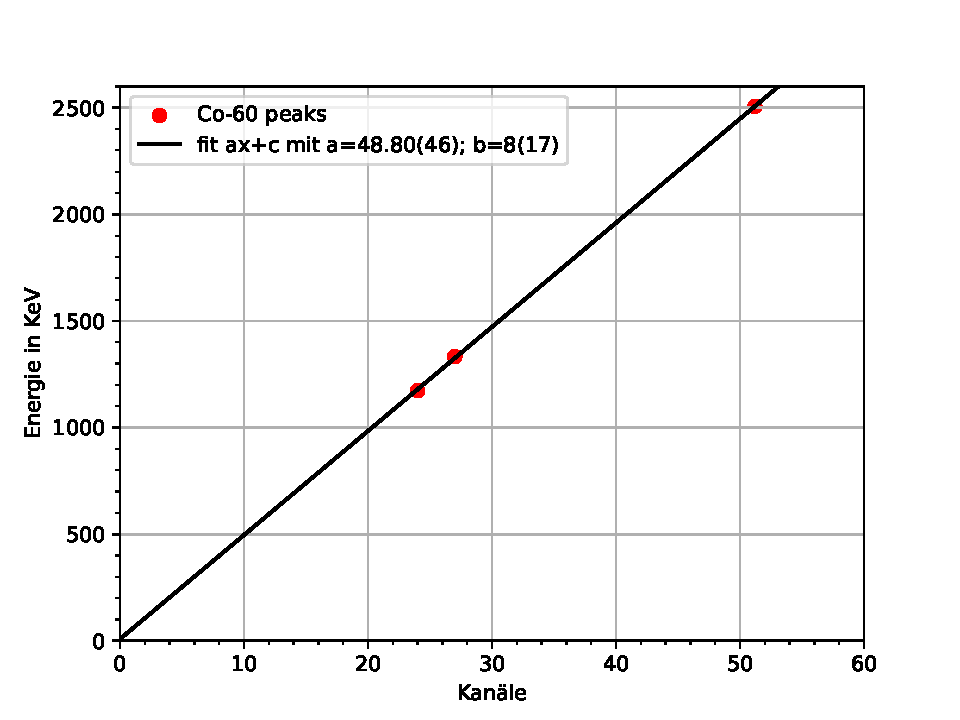
\includegraphics[width=\textwidth]{Plots/Cobalt-Kalib.pdf}
        \caption{Kalibrierungskurve für Höhenstrahlung}
        \label{fig:Höhenkalib}
    \end{figure}

    \begin{figure}[!h]
        \centering
        \includegraphics[width=\textwidth]{Plots/Höhenstrahlung.pdf}
        \caption{Spektrum der Höhenstrahlung}
        \label{fig:Höhenspekt}
    \end{figure}

    \begin{table}
        \centering
        \begin{tabular}{c|c}
            
            Kanalbereich & Anzahl der Ereignisse\\ \hline
            100 - 200 & 1687.0\\  \hline
            200 - 300 & 1235.0\\ \hline
            300 - 400 & 1099.0\\ \hline
            400 - 500 & 1033.0\\ \hline
            500 - 600 & 1055.0\\ \hline
            600 - 700 & 1356.0\\ \hline
            700 - 800 & 1149.0\\ \hline
            800 - 900 & 590.0\\ \hline
            900 - 1000  & 274.0\\ \hline

            
        \end{tabular}
        \caption{Ereignisse in den einzelnen Kanalbereichen}
        \label{tab:Höhenereig}
    \end{table}

    
    \section{Fragen}
    \begin{enumerate}
        \item Ein Elektronvolt ist die Menge an kinetischer Energie, die ein einzelnes Elektron gewinnt oder verliert, wenn es sich von der Ruhe aus durch einen elektrischen Potentialunterschied von einem Volt im Vakuum beschleunigt.
        Ein kosmisches Teilchen mit einer Energie von $4 \cdot 10^{12}$ GeV hat eine Energie von $4 \cdot 10^{12} \cdot 10^9$ eV oder $4 \cdot 10^{21}$ eV. Da 1 eV = $1.602 \times 10^{-19}$ J ist3, hat das kosmische Teilchen eine Energie von $4 \cdot 10^{21} \cdot 1.602 \times 10^{-19}$ J oder etwa $6.408 \times 10^2$ J.        
        Zum Vergleich: Eine AA-Batterie enthält etwa 4 Wattstunden oder etwa 14.400 Joule an Energie.
        \item Die Peaks in einem Experiment haben eine Breite aufgrund von verschiedenen Faktoren wie der Auflösung des Detektors, der statistischen Natur der Messungen und der Breite der Energieverteilung der emittierten Strahlung.
        Nicht alle $\gamma$-Quanten einer bestimmten Energie werden in einem einzigen Kanal gezählt, da die Energieauflösung des Detektors nicht unendlich ist und es immer eine gewisse Unschärfe in der Messung gibt.
        Die Halbwertsbreite (engl. Full Width at Half Maximum, FWHM) ist ein Maß für die Breite eines Peaks in einem Spektrum. Es wird definiert als die Breite des Peaks bei der halben Höhe des Maximums.
        \item Das $Na^{22}$-ZerfallsSpektrum besteht aus zwei Hauptpeaks. Der erste Peak bei 511 keV entsteht durch die Annihilation von Elektronen und Positronen. Der zweite Peak bei 1.27 MeV entsteht durch einen Kernenergieübergang.
        \item Die X-Ray Transition Energies der K Linie von Blei liegen etwa in dem Bereich 72-88 keV \cite{blei}. Durch die Strahlung kann das Blei angeregt werden, wodurch es selber Gamma-Quanten in diesem Energiebereich aussendet.
        \item Die statistische Unsicherheit $\Delta n = \sqrt{n}$ bedeutet, dass die Unsicherheit in der Anzahl der Zerfälle proportional zur Quadratwurzel der Anzahl der Zerfälle ist. Für hohe Zählraten bedeutet dies, dass die relative Unsicherheit $\frac{\Delta n}{n} = \frac{1}{\sqrt{n}}$ kleiner wird. Dies bedeutet, dass die Messung genauer wird, je mehr Zerfälle gezählt werden.
        \item Dieses Verhalten kann durch die Erzeugung von Tochterkernen erklärt werden. Wenn ein langlebiger radioaktiver Kern wie Ra zerfällt, erzeugt er Tochterkerne, die ebenfalls radioaktiv sein können. Diese Tochterkerne können ihrerseits zerfallen und weitere Tochterkerne erzeugen.
        Wenn das Präparat frisch gereinigt wurde, gibt es zunächst keine Tochterkerne. Die Aktivität des Präparats steigt daher zunächst an, da immer mehr Tochterkerne erzeugt werden. Sobald jedoch eine ausreichende Anzahl von Tochterkernen vorhanden ist, beginnen diese ebenfalls zu zerfallen. Dies führt dazu, dass die Aktivität des Präparats nahezu konstant bleibt, da die Erzeugung neuer Tochterkerne durch den Zerfall der vorhandenen Tochterkerne ausgeglichen wird.
        Erst wenn die Anzahl der langlebigen Ra-Kerne signifikant abnimmt, beginnt sich die Abnahme der Aktivität durch das Zerfallsgesetz bemerkbar zu machen.
        \item \begin{itemize} \item $\alpha$-Strahlung sind Heliumkerne mit einer geringen Reichweite und einer hohen Ionisationsfähigkeit. Sie können leicht durch eine Schicht aus Papier oder Kunststoff abgeschirmt werden. \item $\beta$-Strahlung sind Elektronen oder Positronen mit einer mittleren Reichweite und einer mittleren Ionisationsfähigkeit. Sie können durch einige Millimeter aus Aluminium oder Kunststoff abgeschirmt werden. Blei ist manchmal unwirksam, da es sekundäre Strahlung erzeugen kann. \item $\gamma$-Strahlung sind hochenergetische Photonen mit einer langen Reichweite und einer geringen Ionisationsfähigkeit. Sie können nur durch dicke Schichten aus Blei oder Beton abgeschirmt werden. Die Abschirmung hängt von der Dicke und dem Material des Absorbers ab. \item Kosmische Strahlung sind hochenergetische Teilchen aus dem Weltraum mit einer sehr langen Reichweite und einer sehr hohen Ionisationsfähigkeit. Sie können nicht vollständig abgeschirmt werden, aber einige Strategien zur Verringerung der Exposition sind: im Inneren bleiben, Fenster und Türen schließen, sich duschen oder exponierte Körperteile mit einem feuchten Tuch abwischen, abgefülltes Wasser trinken und Lebensmittel in versiegelten Behältern essen, Magnete oder andere Materialien verwenden, um die Strahlung abzulenken oder zu absorbieren, die individuellen Dosen überwachen und die Missionsdauer begrenzen, Teilchenbeschleuniger verwenden, um die Strahlenwirkung zu simulieren und zu testen. \end{itemize}
        \item Die Linien bei 2615 keV, 2104 keV und 1593 keV sind Gammastrahlen, die von Thorium und seinen Zerfallsprodukten emittiert werden. Thorium ist ein natürlich radioaktives Element, das Gammastrahlen abgibt, wenn es zerfällt \cite{thorium_gamma_spectrometry} \cite{radionuclide_basics_thorium}. Die Gammastrahlen haben verschiedene Energien, die von den Übergängen der angeregten Kerne abhängen \cite{gamma-ray_spectrometer}. Die Linien bei 2615 keV und 1593 keV stammen von Thallium-208, einem Zerfallsprodukt von Thorium-232 \cite{analysis_of_uranium_and_thorium_lines} \cite{the_th-232_decay_chain}. Die Linie bei 2104 keV stammt von Blei-212, einem weiteren Zerfallsprodukt von Thorium-232 \cite{the_th-232_decay_chain}.
        \item \begin{enumerate} \item Ein $\gamma$-Quant fällt in den NaI-Kristall und löst ein Photoelektron aus einem Atom des Kristalls aus. \item Das Photoelektron erzeugt weitere Elektronen durch Ionisation. Die Sekundärelektronen regen den dotierten Thallium-Teil des Kristalls an, der niederenergetische Photonen aussendet. \item Die Photonen treffen auf die Photokathode des Photomultipliers und lösen Photoelektronen aus. Diese Elektronen werden durch eine Reihe von Dynoden verstärkt, die jeweils eine höhere Spannung als die vorherige haben. \item Am Ende des Photomultipliers entsteht ein elektrischer Impuls, der proportional zur Energie des ursprünglichen $\gamma$-Quants ist. \item Der Impuls wird an das Messgerät weitergeleitet und in einen Kanal auf dem Bildschirm gezählt. Der Kanal entspricht der Energie des $\gamma$-Quants. \end{enumerate}
    \end{enumerate}

    \bibliographystyle{plain}
    \bibliography{literature}

\end{document}